\setcounter{section}{28}
\section{Топологическая сортировка ориентированного ациклического графа: определение и алгоритм поиска (с доказательством корректности).}
\par Топологическая сортировка ориентированного ациклического графа $G(V,E)$ представляет собой упорядочивание вершин таким образом, что для любого ребра $(u,v) \in E$ номер вершины $u$ меньше номера вершины $v$.
\par Предположим, что граф ацикличен, т.е. решение существует. Что делает обход в глубину? При запуске из какой-то вершины $v$ он пытается запуститься вдоль всех рёбер, исходящих из $v$. Вдоль тех рёбер, концы которых уже были посещены ранее, он не проходит, а вдоль всех остальных — проходит и вызывает себя от их концов.
\par Таким образом, к моменту выхода из вызова $DFS(v)$ все вершины, достижимые из $v$ как непосредственно (по одному ребру), так и косвенно (по пути) — все такие вершины уже посещены обходом. Следовательно, если мы будем в момент выхода из $DFS(v)$ добавлять нашу вершину в начало некоего списка, то в конце концов в этом списке получится топологическая сортировка.
\lstinputlisting[language=C++,
emph={int,char,double,float,unsigned},
emphstyle={\color{blue}}
]{code/29-31_topsort.cpp}
\par \textbf{Корректность:} $\blacktriangle$ Покажем, что если $(u,v) \in E$, то $u$ выведется раньше $v$. $u$ выведется раньше чем $v \Leftrightarrow tout[v]<tout[u]$ Рассмотрим 2 случая
\begin{enumerate}
    \item $v$ была замечена DFSом раньше чем $u$. Тогда к моменту выхода из $v$ вершина $u$ все еще не посещена, иначе нашелся бы цикл $\Rightarrow tout[v]<tout[u]$
    \item $u$ была замечена раньше чем $v$. Тогда мы перейдем по ребру $(u,v)$ в $v$, а до выхода из $u$ необходимо выйти из всех вершин, в которые мы попали из нее (по лемме о белых путях) $\Rightarrow tout[v]<tout[u] \: \blacksquare$
\end{enumerate}
\par \textbf{Асимптотика:} $O(n+m)$ (dfs проходит каждому ребру и вершине по 1 разу. Сортировку tout можно сделать прям в dfs идею см. в билете 31)

\setcounter{section}{29}
\section{Отношение сильной связности между вершинами. Компоненты сильной связности. Сильно связный граф.}
\par \textbf{Определение:} В ориентированном графе вершины $u,v$ - \textit{сильно связаны}, если из $u$ есть путь в $v$ и из $v$ есть путь в $u$.
\par \textbf{Утверждение:} сильная связность является отношением эквивалентности
\par $\blacktriangle$ Рефлексивность и симметричность очевидны из определения. Транзитивность получается из того что просто склеиваем пути $\blacksquare$
\par \textbf{Определение:} Классы эквивалентности относительно отношения сильной связности, на которые разбивается граф, называются \textit{компонентами сильной связности}.
 \par \textbf{Определение:} Ориентированный граф \textit{сильно связен}, если для каждой вершины все остальные вершины достижимы из нее.
 \begin{figure}[h]
\hspace{-4ex} \begin{minipage}[h]{0.3\linewidth}
\center{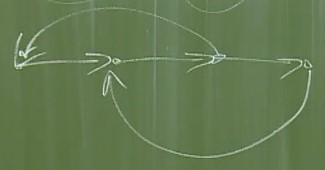
\includegraphics[scale=0.3]{images/29-31_kss.jpg}}
\end{minipage}
\hfill
\hspace{-4ex} \begin{minipage}[h]{0.7\linewidth}
 \par \textbf{Пример:} компонента сильной связности (сама является сильно связным графом)
\end{minipage}
\end{figure}

\setcounter{section}{30}
\section{Алгоритм Косарайю. Корректность и время работы.}
\begin{enumerate}
    \item Выполним $DFS$, вычисляющий для каждой вершины время выхода $DFS$ из нее (этот массив обозначим за $p$).
    \item Строим граф $H$ с инвертированными ребрами
    
    \item Выполняем $DFS$ на $H$, перебирая вершины в порядке убывания $p(u)$.
\end{enumerate}
\lstinputlisting[language=C++,
emph={int,char,double,float,unsigned},
emphstyle={\color{blue}}
]{code/29-31_kosarayu.cpp}
\begin{figure}[h]
\center{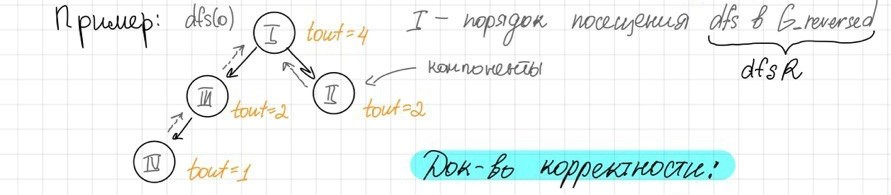
\includegraphics[width=\linewidth]{images/29-31_kosarayu.jpg}}
\end{figure}
\par \begin{itemize}
    \item[$\blacktriangle$ 1.] Если $v$ - вершина с максимальным tout в своей КСС, то $reversed\_dfs(v)$ посетит как минимум всю эту КСС (так как все остальные вершины из нее еще не used) $\Rightarrow$ целиком содержит эту КСС, так как $reversed\_dfs$ проходит по всем вершинам, из которых достижимо $v$ в исходном графе
    \item[2.] Покажем, что не посетили больше чем одну КСС. Пусть $u,v$ лежат в разных КСС. Тогда имеет место один из двух случаев
    \begin{itemize}
        \item нет путей из $u$ в $v$ и из $v$ в $u$
        \par Очевидно, что в этом случае ни одна из вершин не достижима из другой ни по прямым, ни по инвертированным ребрам $\Rightarrow$ алгоритм причислит их к разным КСС
        \item Есть путь из $u$ в $v$, но нет пути из $v$ в $u$ (симметричный случай доказывается аналогично)
        \par Тогда $tout[u]>tout[v]$ (доказательство аналогично доказательству корректности в топологической сортировке, билет 29). Значит $reversed\_dfs(u)$ запустится раньше чем от $v$. Так как по предположению из $v$ в $u$ нет пути, то $reversed\_dfs(u)$ не попадет в $v$. Но тогда $reversed\_dfs(v)$ уже не попадет в $u$, так как она $used \Rightarrow$ алгоритм причислит их к разным КСС $\blacksquare$
    \end{itemize}
\end{itemize}
\par \textbf{Асимптотика:} $O(n+m)$ (обходим все вершины и ребра по одному разу dfsом, потом по одному разу reversed\_dfsом)